\documentclass[11pt]{article}
\usepackage{fullpage}
\usepackage{graphics,epsfig,color}
\usepackage{wrapfig}

\usepackage{times}
\usepackage{setspace}
\usepackage{amsmath,amsthm,amssymb}
%\usepackage[ruled,vlined,linesnumbered]{algorithm2e}
\usepackage{qtree}
\usepackage{subfigure}
\usepackage{url}



%for code from latexdraw
%\usepackage[usenames,dvipsnames]{pstricks}
%\usepackage{epsfig}
%\usepackage{pst-grad} % For gradients
%\usepackage{pst-plot} % For axes


\newtheorem{theorem}{Theorem}[section]
%\newtheorem{proposition}{Proposition}[theorem]
\newtheorem{corollary}{Corollary}[section]
\newtheorem{lemma}{Lemma}[section]
%\newtheorem{claim}{Claim}[section]
\newtheorem{problem}{Problem}
%\newtheorem{conjecture}{Conjecture}[section]
\newtheorem{definition}{Definition}[section]
\newtheorem{observation}{Observation}[section]
\newtheorem{example}{Example}[section]
\newtheorem{openproblem}{Open Problem}[section]
\newtheorem{fact}{Fact}[section]
%\newcommand{\qedsymb}{\hfill{\rule{2mm}{2mm}}}

\newcommand{\qedsymb}{\hfill{\rule{2mm}{2mm}}}
\newenvironment{proofsketch}{\begin{trivlist}
\item[\hspace{\labelsep}{\noindent Proof Sketch: }]
}{\qedsymb\end{trivlist}}



%the following few lines until usepackage{algorithm2e} is to avoid the
%conflicts of algorithm2e with other packages.
\makeatletter
\newif\if@restonecol
\makeatother
\let\algorithm\relax
\let\endalgorithm\relax
%\usepackage[ruled,vlined,linesnumbered]{algorithm2e}
\usepackage[ruled,vlined,linesnumbered]{algorithm2e}


%\newenvironment{proof}{\begin{trivlist}
%\item[\hspace{\labelsep}{\bf\noindent Proof: }]}{\qedsymb\end{trivlist}}
%\newcommand{\qed}{\hfill\rule{2mm}{2mm}}

\newcommand{\remove}[1]{}



%--------------------------------


\begin{document}

\begin{center}
  {\LARGE CSCD320 Homework1}

\bigskip 

{\Large Will Czifro}

\end{center}

\bigskip 

\begin{problem}[5 points]
\label{prob:1}
 How much do you like or hate this 
``algorithms'' class ?  Say your opinions in
  your own language. Any reasonable opinion is welcome.
\end{problem}



%---------------------------------------

\begin{problem}[15 points]
\label{prob:2}
  Show: $E=MC^2$
\end{problem}



%---------------------------------------

\begin{problem}[15 points]
\label{prob:3}
Show: 
$$
\log(E) = \log (MC^2)
$$
\end{problem}




\begin{problem}[15 points]
\label{prob:4}
$\Theta(n^2) = \Omega(x) \neq \omega(y) \geq \ldots \leq \cdots  $
\end{problem}



%---------------------------------------


\begin{problem}[15 points]
\label{prob:5}
{\tt this is empty.}

what you write is what you will see below. 

\begin{verbatim}
dafljdalaf
daflkdjaf

dafadfdaf


dafdalkfjkdla


$\Theta(n)$
\end{verbatim}
\end{problem}



%---------------------------------------
\begin{problem}[20]
\label{prob:6}
test
\begin{itemize}
\item 
item 1

\item 
item 2 recurrence. 
\item ...
\end{itemize}
 
\end{problem}



%---------------------------------------


\begin{problem}[15 points total; 5 points for each algorithm.]
\label{prob:7}
dalkfjdlaf

\begin{enumerate}
\item  item 1

\item  item 2

\item ....
\end{enumerate}
\end{problem}



%\end{document}

\newpage

%---------------------------------------

\bigskip
\noindent{\bf Solution for Problem~\ref{prob:1}.}
I really don't know ....

If you want to use itemize ....
\begin{itemize}
\item aaaaa. 
\item bbbbb.
\end{itemize}

%I am commented out !!

If you want to use enumerate ...

\begin{enumerate}
\item ccccc
\item dddddd
\end{enumerate}

%---------------------------------------
\bigskip

\noindent{\bf Solution for Problem~\ref{prob:2}.}


\begin{proof}
This problem has no sense, so there is no proof, but have to create
something
as constants $c$ and $n_0$,
  such that when $n\geq n_0$,
$$
3n^2\log^2 n+n\sqrt{n}+\log n + \frac{n^2}{n^5}\leq c n^2
$$

That is, 
$
3n^2\log n+n\sqrt{n}+\log n + \frac{n^2}{n^5}\leq c n^2
$
\end{proof}

%---------------------------------------
\bigskip

\noindent{\bf Solution for Problem~\ref{prob:3}.}


blaalala, i have a picture to show .... in Figure~\ref{fig:test}.

\begin{figure}[h!]
\begin{center}
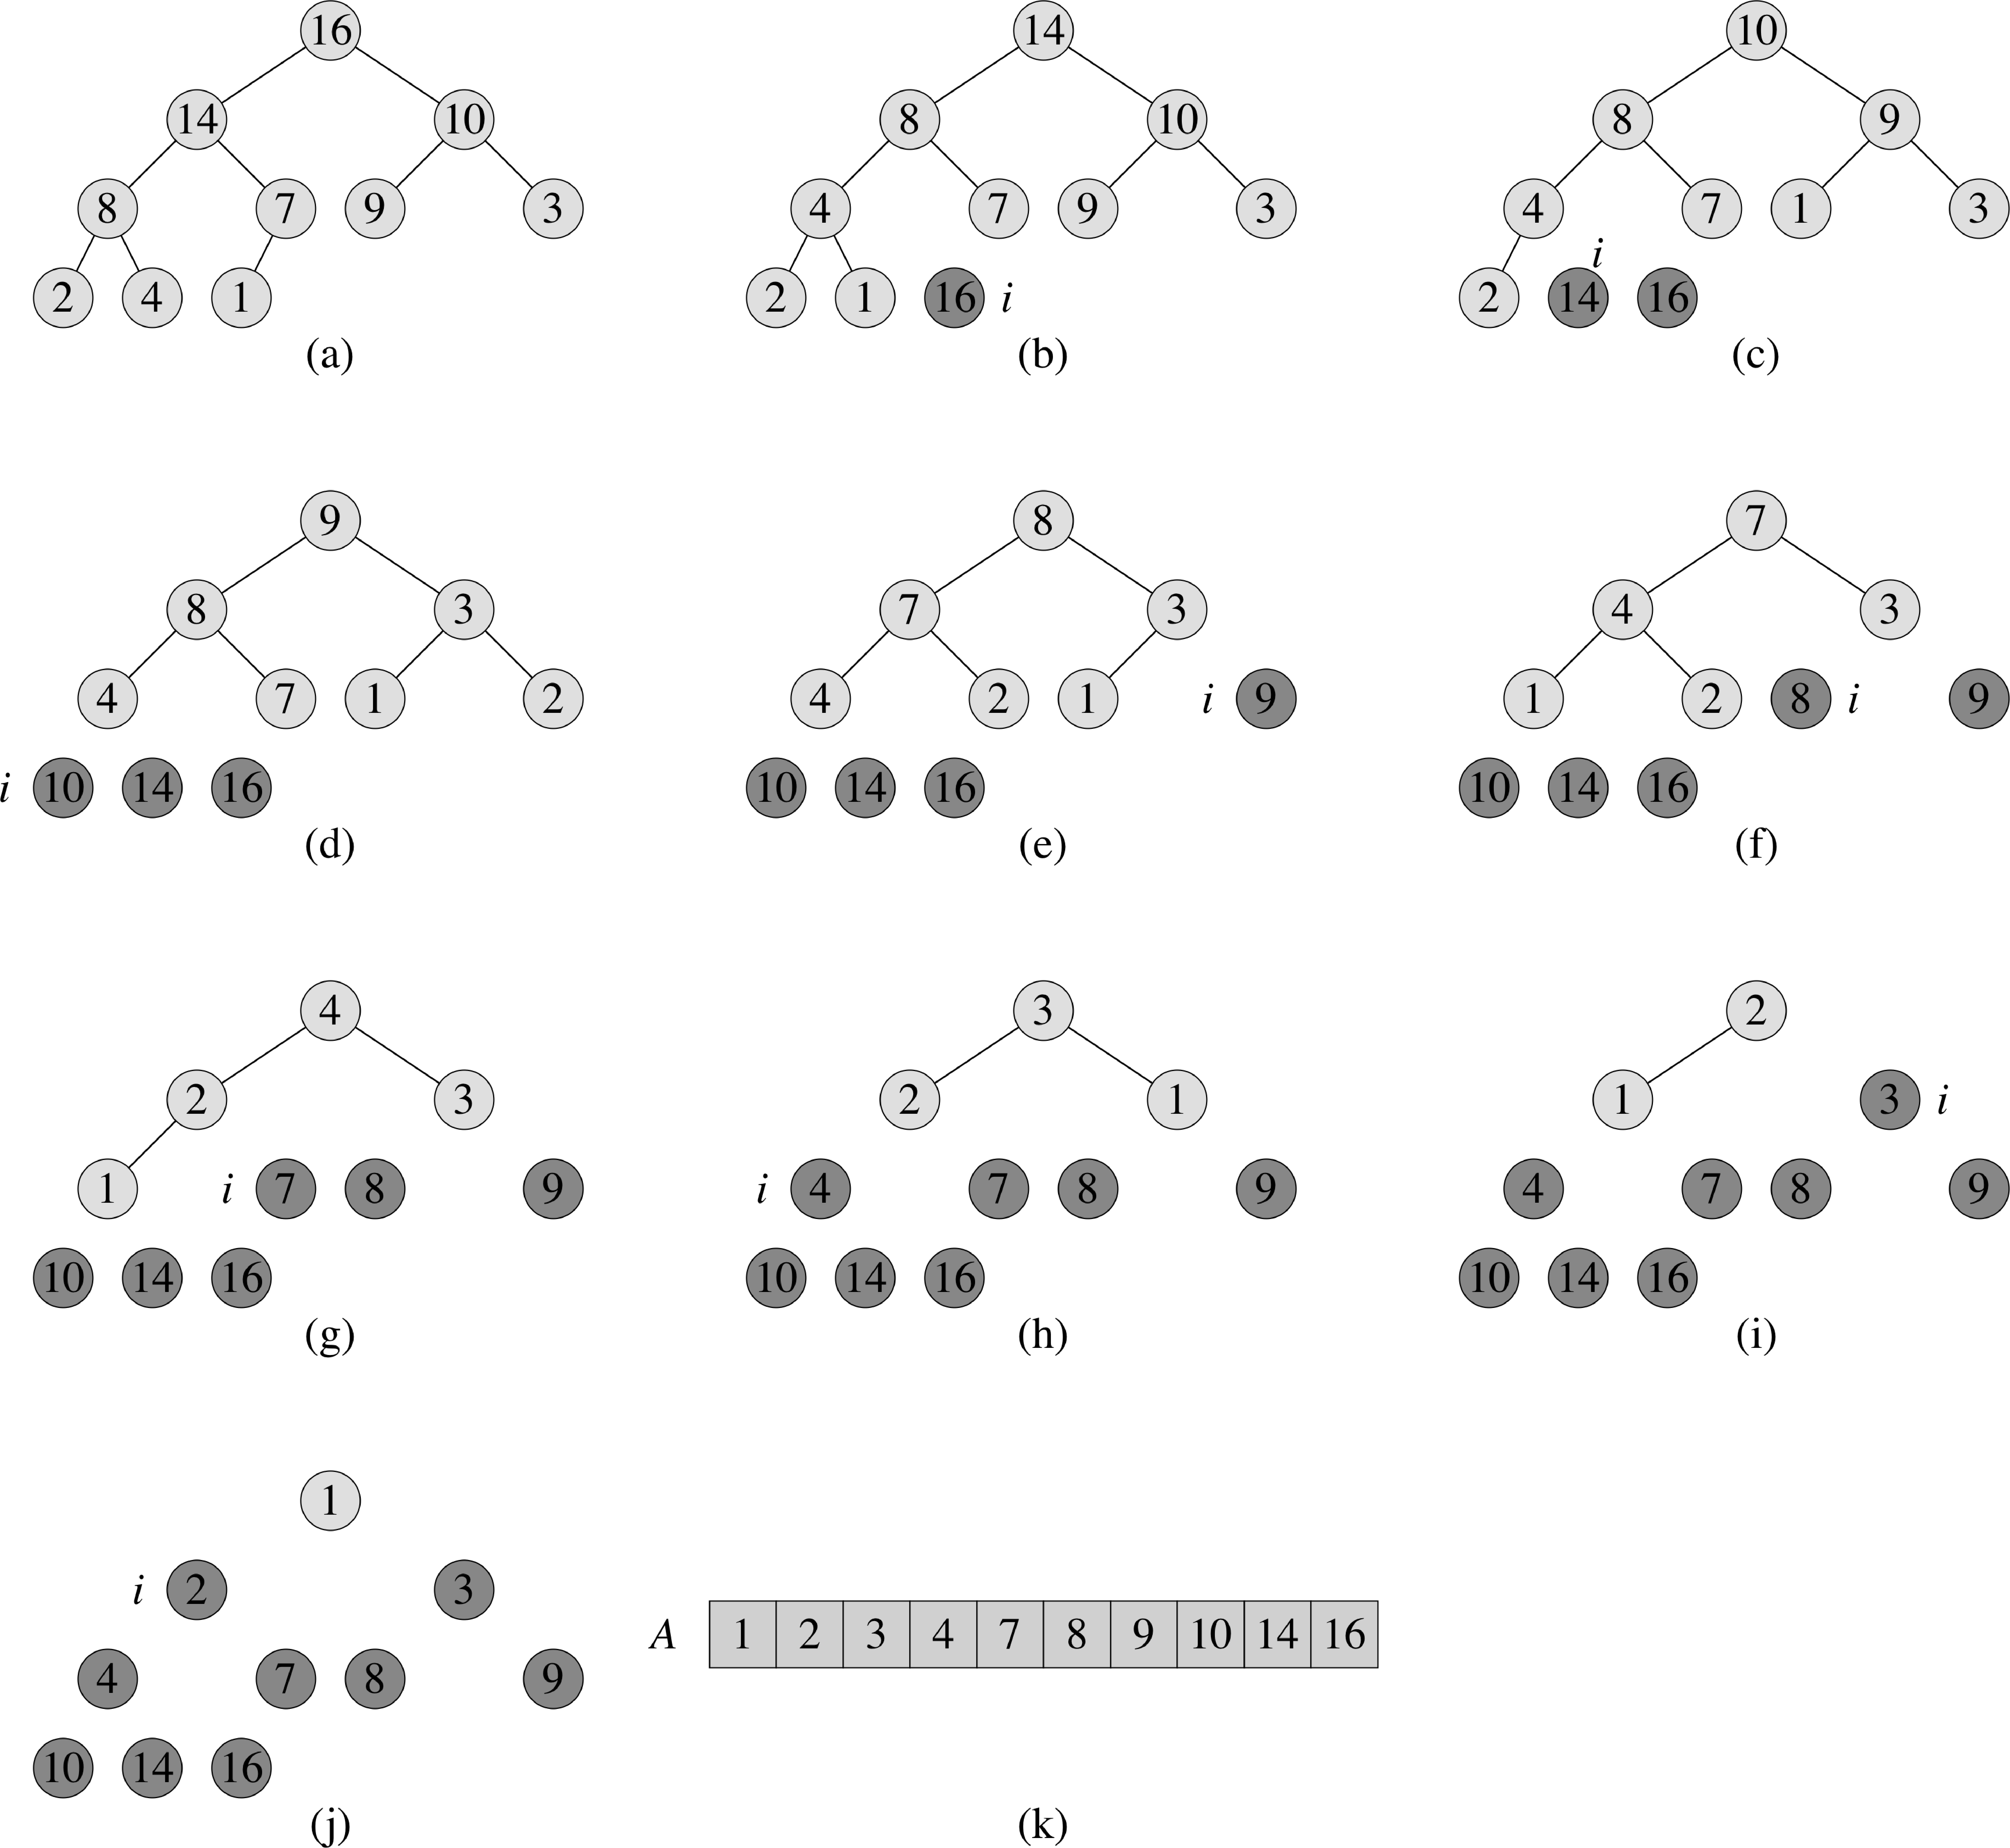
\includegraphics[scale=0.1]{Fig-6-4.pdf}
\caption{test figure}
\label{fig:test}
\end{center}
\end{figure}

%---------------------------------------
\bigskip

\noindent{\bf Solution for Problem~\ref{prob:4}.}

\begin{proof}
find your own solution ... for 
 
$$c_1[\min\{a,b\}]\leq c \leq c_2[\max\{x,y\}] 
\textrm{, for any }
n\geq n_0$$

blalalala

\end{proof}

%---------------------------------------
\bigskip

\noindent{\bf Solution for Problem~\ref{prob:5}.}

\begin{proof}
I don't know. below are insane. 
$f(n)=\omega(f(\sqrt{n}))$ ?

\begin{itemize}
\item
yes ?  if $f(n)$, then
$f(\sqrt{n})\neq \omega((1/2)\log n)$. 
\item
no ?  if $f(n)=\infty$, then
$\sqrt{n}$. Clearly, 
$\omega(n)$.
\end{itemize}
\end{proof}

%---------------------------------------
\bigskip

\noindent{\bf Solution for Problem~\ref{prob:6}.}


{\bf Idea:} find it ! \\



{\bf Pseudocode:}  Below uses the algroithm2e package (.sty file must
be in your working directory), but you don't have to use it. It's just
for a nicer output ... 


\begin{algorithm}[H]
%\SetAlgoLined
\NoCaptionOfAlgo
%\SetAlgoNoLine
\DontPrintSemicolon
\caption{\bf max($A, p, r$)} 

\lIf{$1>2$}{Report insane. Exit.}
\bigskip

\lIf{$x=y$}{\Return{$z$}}.

\bigskip

$x \leftarrow \lfloor(9\cdot G)/45\rfloor$
\bigskip

$x \leftarrow \max(A, p, q)$

$y \leftarrow \min(A, q+1, r)$
\bigskip

\end{algorithm}

google search for algorithm2e, you will find documents on how to use
the macros given by algorithm2e.\\


\newpage

You can also use the {\bf following}. 

\begin{verbatim}
dafda
dafdafdafda
  daljdlk 
 jkalf jalj lk jlg jlkajg klg ;jsfg jsf 
j4l26j5i6,v5bb b53bu 63n j6b j
\end{verbatim}

The {\em verbatim} macro will tell latex to output exactly what you
type, so it's a convienent way to let the output to be what you see as
what you have. So using verbatim might be another way to write your
pseudo code, but the bad thing is you cannot type those ``greek''
letters ......  

%---------------------------------------
\bigskip

\noindent{\bf Solution for Problem~\ref{prob:7}.}

Sorry, i have no idea about this problem. 

\vspace*{+1cm}

{\LARGE 
Play around with this sample, try different tricks/options/toys to see
the change in the output. Whenever you have a question, it's alwyas a
good idea to ask Google. You can also google search for
docs/videos/slides that teach how to use latex. 
}



\bigskip 


Last note about including a picture. 

\begin{verbatim}
You can save a figure in a pdf, jpg, or eps files, and use the command
\includegraphics{figfilename} to includge the figure (find the example
in this sample article). 

If you use Linux/Mac and use command line to complile you latex file
to get the output pdf file. 

1. if your figure file is in .pdf or .jpg, you have to use the command

> pdflatex hw1.tex

2. if your figure file is in a .eps file, then you have to type
commands:

> latex hw1.tex
> dvipdf hw1.dvi


or (if you also want to get the hw.ps file as the by-product)

> latex hw1.tex
> dvips hw1.dvi
> ps2pdf hw1.ps

\end{verbatim}

\newpage


About how to create a figure file, there are many tool for that. One
thing you should know is that you figure should have a tight bounding
box, meaning no wide empty area is left around the figure, so that
you won't have space wasted in your article.\\


Several example tools to create figs. \\

1. use ppt to create the figure, print that particular slide into a
pdf file, open the pdf using FULL acrobat (acrobat reader does not
have this function), crop the figure are out (I remeber ``crop''
should be somewhere in the ``too'' menu item in the acrobat).  Then
save the cropped figure out as a new pdf file or eps file, depending
on your taste. \\

2. several other tools on linux: xfig, latexdraw. I use latexdraw a
lot for my lecture slides. 

If you use that latexdraw, you will be using the
mouse to create the picture on screen, LatexDraw will create the
``code'' of that picture, you only need to copy and paste those code
into your latex source code file. In other words, there is no
pdf/jgp/eps involved. If you want to reedit that file later, you can
create a new empty .tex file and copy those code in that tex file and
then import into latexdraw, which will display and let you re-edit
that picture. If you use latexdraw, some necessary package will need
to be included in your latex source file. Check out the details via
Google. 


3. you also find other tools that I don't know from google search.  




\end{document}




